\documentclass[10pt]{exam}

\usepackage[margin=1in]{geometry}
\usepackage{amsmath}
\usepackage{amssymb}
\usepackage{amsthm}
\usepackage{mathtools}
\usepackage{bm}
\usepackage{stmaryrd}
\usepackage{booktabs}

\usepackage{color}
\usepackage{colortbl}
\definecolor{deepblue}{rgb}{0,0,0.5}
\definecolor{deepred}{rgb}{0.6,0,0}
\definecolor{deepgreen}{rgb}{0,0.5,0}
\definecolor{gray}{rgb}{0.7,0.7,0.7}

\usepackage{hyperref}
\hypersetup{
  colorlinks   = true, %Colours links instead of ugly boxes
  urlcolor     = black, %Colour for external hyperlinks
  linkcolor    = blue, %Colour of internal links
  citecolor    = blue  %Colour of citations
}

\usepackage{listings}
\lstset{
    basicstyle={\ttfamily}
}

%%%%%%%%%%%%%%%%%%%%%%%%%%%%%%%%%%%%%%%%%%%%%%%%%%%%%%%%%%%%%%%%%%%%%%%%%%%%%%%%

\theoremstyle{definition}
\newtheorem{problem}{Problem}
\newtheorem{example}{Example}
\newtheorem{lemma}{Lemma}
\newtheorem{corollary}{Corollary}
\newtheorem{note}{Note}
\newtheorem{defn}{Definition}
\newtheorem{fact}{Fact}
\newtheorem{refr}{References}
\newtheorem{theorem}{Theorem}
\newcommand{\E}{\mathbb E}
\newcommand{\R}{\mathbb R}
\DeclareMathOperator{\nnz}{nnz}
\DeclareMathOperator{\sign}{sign}
\DeclareMathOperator{\determinant}{det}
\DeclareMathOperator{\Var}{Var}
\DeclareMathOperator{\rank}{rank}
\DeclareMathOperator{\prob}{\mathbb P}
\DeclareMathOperator*{\argmin}{arg\,min}
\DeclareMathOperator*{\argmax}{arg\,max}

\newcommand{\Ein}{E_{\text{in}}}
\newcommand{\Eout}{E_{\text{out}}}
\newcommand{\Etest}{E_{\text{test}}}
\newcommand{\I}{\mathbf I}
\newcommand{\Q}{\mathbf Q}
\newcommand{\p}{\mathbf P}
\newcommand{\pb}{\bar {\p}}
\newcommand{\pbb}{\bar {\pb}}
\newcommand{\pr}{\bm \pi}

\newcommand{\trans}[1]{{#1}^{T}}
\newcommand{\loss}{\ell}
\newcommand{\w}{\mathbf w}
\newcommand{\wstar}{{\w}^{*}}
\newcommand{\x}{\mathbf x}
\newcommand{\y}{\mathbf y}
\newcommand{\lone}[1]{{\lVert {#1} \rVert}_1}
\newcommand{\ltwo}[1]{{\lVert {#1} \rVert}_2}
\newcommand{\lp}[1]{{\lVert {#1} \rVert}_p}
\newcommand{\linf}[1]{{\lVert {#1} \rVert}_\infty}
\newcommand{\lF}[1]{{\lVert {#1} \rVert}_F}

\newcommand{\mH}{m_{\mathcal H}}
\newcommand{\dvc}{{d_{\text{VC}}}}
\newcommand{\HH}[1]{\mathcal H_{\text{#1}}}
\newcommand{\Hbinary}{\HH_{\text{binary}}}
\newcommand{\Haxis}{\HH_{\text{axis}}}
\newcommand{\Hperceptron}{\HH_{\text{perceptron}}}


\newcommand{\ignore}[1]{}

%%%%%%%%%%%%%%%%%%%%%%%%%%%%%%%%%%%%%%%%%%%%%%%%%%%%%%%%%%%%%%%%%%%%%%%%%%%%%%%%

\begin{document}


\begin{center}
{
\Huge
Model Zoo
}
\end{center}

\section{Introduction}

Scikit-learn implements many different classification models.
The VC dimension gives us a generic tool for understanding the generalization performance of all of these models.
These notes will give a high level overview of the most important variants of these models and their VC dimension.

None of this information is in the textbook.
Citations are provided for all the information,
but you're not expected to look at the original sources.
There are two goals for including this material:
(1) so that you can use this material to determine which models to use in practice;
(2) so that you get a sense of what the state of the art in machine learning theory is.

There's one last section for us to cover in the textbook
(4.3.2 model selection),
but it makes sense for us to have a large set of example models to think about before covering this section.

\section{Models}

\begin{center}
    \hspace*{-0.75in}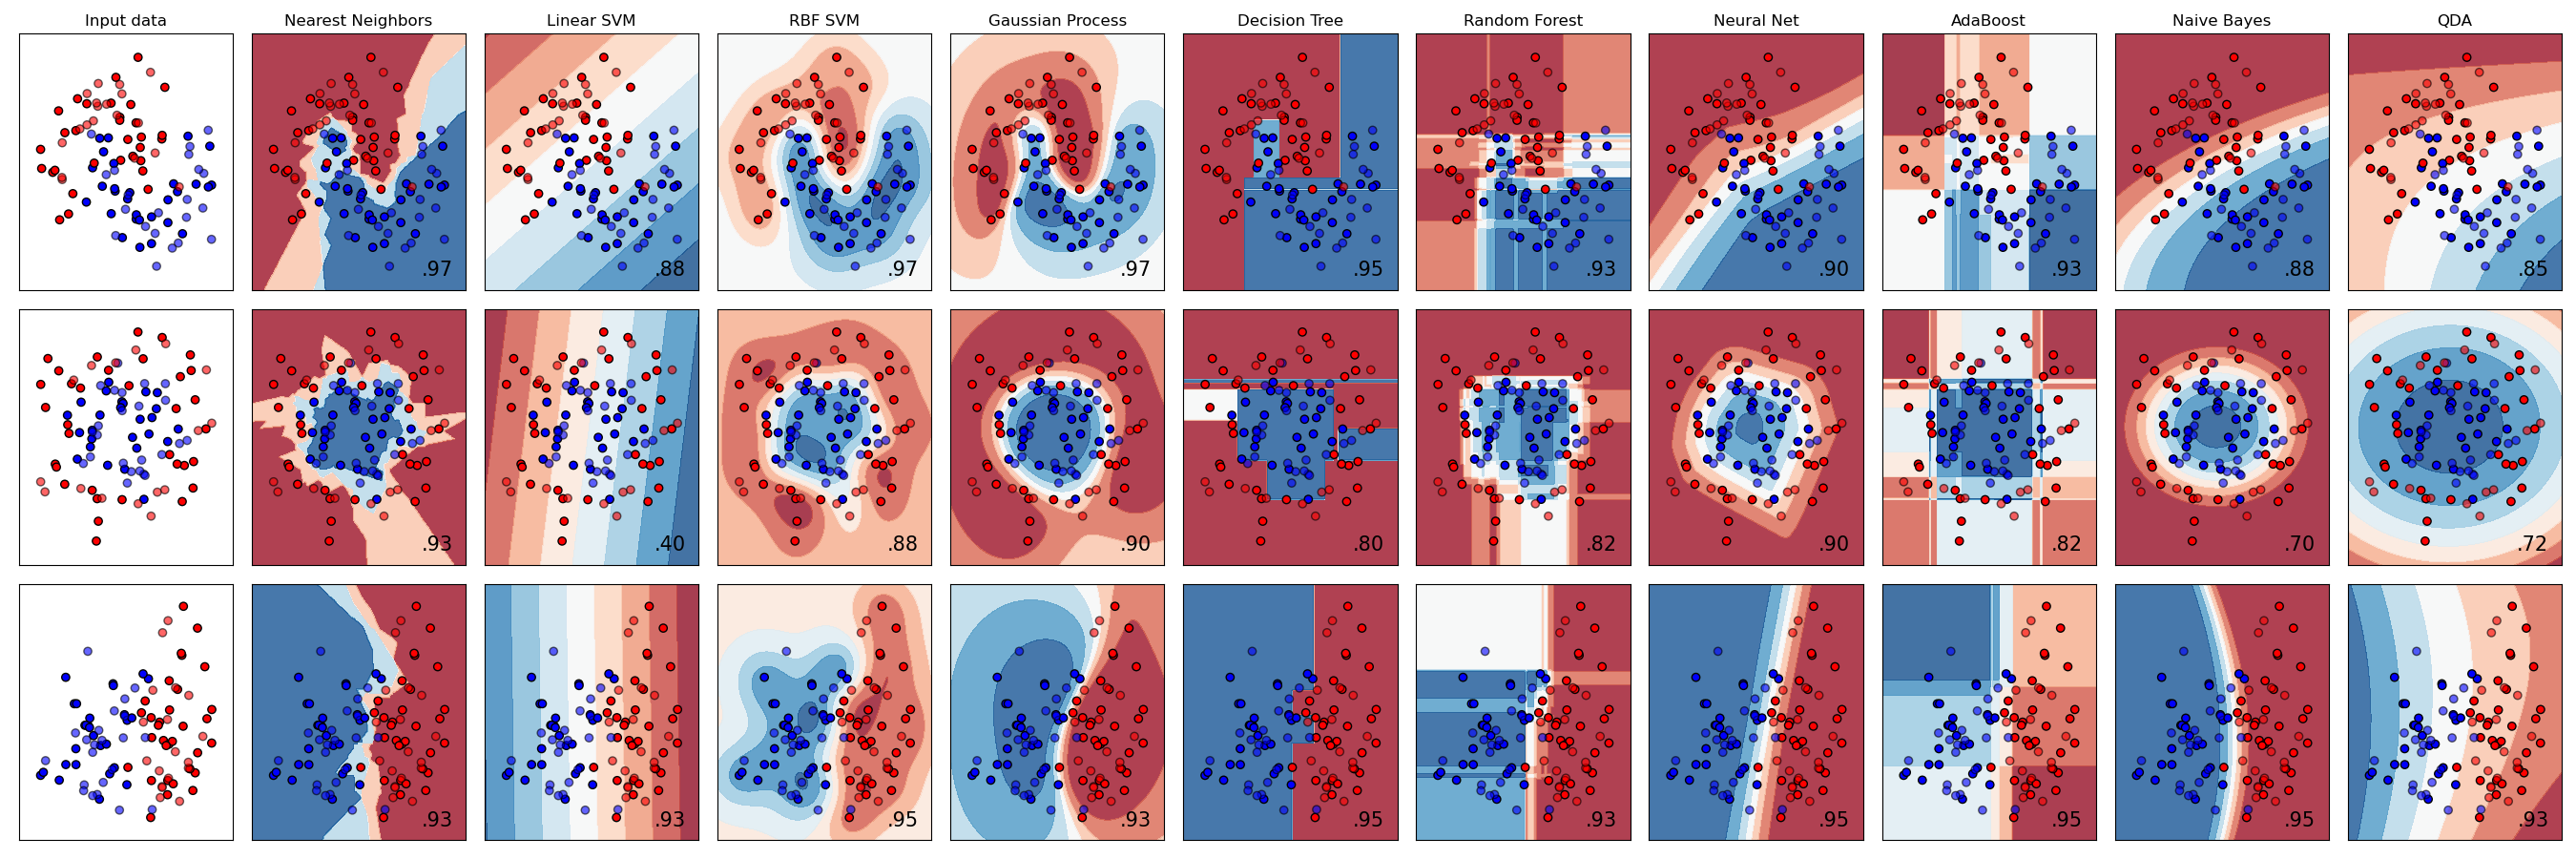
\includegraphics[width=8in]{sphx_glr_plot_classifier_comparison_001}
    \small
    Source: \url{https://scikit-learn.org/stable/auto_examples/classification/plot_classifier_comparison.html}
\end{center}
\newpage
\subsection{Linear/Quadratic Models}

Scikit learn implements the following linear models:

\begin{code}
sklearn.discriminant_analysis.LinearDiscriminantAnalysis()
sklearn.linear_model.LogisticRegression()
sklearn.linear_model.Perceptron()
sklearn.linear_model.SGDClassifier()
sklearn.linear_model.PassiveAggressiveClassifier()
sklearn.svm.LinearSVC
\end{code}

%\begin{fact}
    Recall that a model refers to a hypothesis class and a training algorithm.
    All linear models use the hypothesis class of halfspaces, and all quadratic models use halfspaces with a 2nd degree polynomial kernel.
    Therefore, the VC dimension of all linear models is $\Theta(d)$ and all quadratic models is $\Theta(d^2)$.
    This immediately implies that the generalization error is
    \begin{equation}
        \Eout = \Ein + O\bigg(\sqrt{\frac{d\log N}{N}}\bigg)
    \end{equation}
    for linear models and
    \begin{equation}
        \Eout = \Ein + O\bigg(\sqrt{\frac{d^2\log N}{N}}\bigg)
    \end{equation}
    for quadratic ones.

    The only difference between these models and logistic regression is the training algorithm.
    Models like \lstinline{sklearn.discriminant_analysis.LinearDiscriminantAnalysis} and \lstinline{class sklearn.naive_bayes.GaussianNB} make parametric assumptions on the underlying data and minimize $\Ein$ under those assumptions.
    Logistic regression and SVMs are able to minimize $\Ein$ without any assumptions, however, so they ``usually'' have better training error.

    In practice, practitioners almost always use logistic regression or SVMs to optimize linear/quadratic hypothesis spaces because the training error is smaller and the generalization error is the same.

%\end{fact}

    \vspace{5in}
\begin{note}
    A common interview question is to explain the assumptions behind some of these ``bad'' models like naive bayes or linear discriminant analysis.
    I won't ask you to do that for this class.
\end{note}

\newpage
\begin{problem}
    A colleague is using quadratic discriminant analysis to solve a machine learning problem.
    Provide simple suggestions on how they could improve classification accuracy in the following situations.
    \begin{enumerate}
        \item
            They are overfitting.
            \vspace{4in}
        \item
            The training error $\Ein$ is large.
    \end{enumerate}
\end{problem}

%\vspace{4in}
%\begin{problem}
    %What is the VC dimension of 
%\end{problem}

\newpage
\subsection{Multi Layer Perceptron (MLP)}

Recall that the class of binary halfspaces is
\begin{equation}
    \HH{} = \bigg\{ \x \mapsto \sign(\trans\w \x) : \w : \R^{d'} \bigg\}
\end{equation}
and it is common to adjust the VC-dimension of the problem by applying a feature map
$\Phi : \R^d \to \R^{d'}$ to get the hypothesis class
\begin{equation}
    \HH{} = \bigg\{ \x \mapsto \sign(\trans\w \Phi(\x)) : \w : \R^{d'} \bigg\}
    .
\end{equation}
In logistic regression, we fix the $\Phi$ function in advance and learn only the $\w$ vector.

The idea of the MLP is to also learn the $\Phi$ function from the data.
In a 1-layer MLP, we set
\begin{equation}
    \Phi(\x) = \sigma ( W_1 \x)
\end{equation}
where $W_1 : \R^{d'\times d}$,
and $\sigma : \R \to \R$ is called the \emph{activation function} and is applied element-wise to $W_1\x$.
The $W_1$ matrix is learned from the data (typically via stochastic gradient descent) at the same time as the $\w$ vector.
In the $i$-layer perceptron, the $\Phi$ function is recursively defined to be
\begin{equation}
    \Phi^{(i)}(\x) =
    \begin{cases}
        \sigma (A_1 \x) & \text{if}~i = 1 \\
        \sigma (A_i \Phi^{(i-1)}(\x)) & \text{otherwise}
    \end{cases}
\end{equation}
where each matrix $A_i : \R^{d_i \times d_{i-1}}$ and $d_0 = d$ and $d_i = d'$.
The value $i$ is called the \emph{depth} of the neural network or the \emph{number of layers} of the network, and the value of $d_i$ is called the width of the $i$th layer.


\vspace{4in}
\begin{note}
    The MLP is a special case of a \emph{neural network}.
    TensorFlow/PyTorch are libraries from Google/Facebook for implementing neural networks that give much more control than scikit-learn.

    TensorFlow has a good visualization of MLPs at:
    \url{https://playground.tensorflow.org}
\end{note}

\newpage
\begin{theorem}[universal approximation]
    Let $g$ be the ERM hypothesis for the 1-layer MLP hypothesis class.
    Then,
    \begin{equation}
        \lim_{d_1\to\infty} \Ein(g) = 0
        .
    \end{equation}
\end{theorem}

\begin{theorem}
    %If $\sigma$ is the identity function, then the VC-dimension of the $k$-layer MLP is
    %\begin{equation}
        %\dvc = \min_{i\in[k]} d_i.
    %\end{equation}
    Define
    \begin{align}
        \label{eq:E}
        E &= \prod_{i=1}^k d_i d_{i-1} = d'd \prod_{i=1}^{k-1} d_i^2.
        \\
        V &= \prod_{i=1}^k d_i
    \end{align}
    The VC-dimension of the $k$-layer MLP with the identity activation function is
    \begin{equation}
        \Theta(d)
        .
    \end{equation}
    The VC-dimension of the $k$-layer MLP with the $\sigma=\sign$ activation function is
    \begin{equation}
        %\dvc = \tilde O\bigg(d'd \prod_{i=1}^{k-1} d_i^2 \bigg)
        \dvc = O(E \log E)
        .
    \end{equation}
    With the $\sigma=\tanh$ activation function, the tightest known bounds on the VC dimension are
    \begin{align}
        \dvc = \Omega(E^2) \quad\text{and}\quad
        \dvc = O(V^2 E^2)
        .
    \end{align}
\end{theorem}

\begin{proof}
    See Section 20.4 of \emph{Understanding Machine Learning: From Theory to Algorithms}.
\end{proof}

\begin{theorem}
    Let $E$ be defined as in Equation \eqref{eq:E} above.
    Then the VC dimension of neural networks with the ReLU (hinge loss) activation function is upper bounded by
    \begin{equation}
        \dvc = O(Ek\log(E))
    \end{equation}
    and lower bounded by
    \begin{equation}
        \dvc = \Omega(Ek\log(E/k)).
    \end{equation}
\end{theorem}

\begin{proof}
    See ``Nearly-tight VC-dimension and pseudodimension bounds for piecewise linear neural networks'', COLT 2017.
\end{proof}

\begin{fact}
    The optimization problem for neural networks is convex only when the activation function $\sigma$ is the identity function.
    Optimization is therefore not guaranteed to lead to a global minimum.
\end{fact}

%\begin{fact}
    %Unlike logistic regression, neural networks are non-convex.
%\end{fact}

\newpage
\begin{problem}
    You are training a \lstinline{sklearn.neural_network.MLPClassifier} model with the hyperparameter \lstinline{activation} set equal to \lstinline{relu} on 1000 dimensional data.
    You have the choice of setting the \lstinline{hidden_layer_sizes} hyperparameter to either (a) \lstinline{[10,10,10]} or (b) \lstinline{[100]}.
    \begin{enumerate}
        \item Which choice is more likely to overfit the data?
            \vspace{3in}
        \item Which choice will likely require a larger value of \lstinline{alpha}?
            \vspace{3in}
    \end{enumerate}
\end{problem}

\newpage
\begin{problem}
    You have successfully trained a \lstinline{sklearn.neural_network.MLPClassifier} model with \lstinline{hidden_layer_sizes} equal to \lstinline{[100,100]} in order to predict whether a user will click on an advertisement.
    The model is neither overfitting nor underfitting the data,
    and so you have successfully tuned all the hyperparameters of this model into their optimal configuration.

    Your colleagues in the marketing department have collected more data, however, and so are requesting a new model be trained that is more accurate.
    The new dataset is twice the size of the old dataset.

    \begin{enumerate}
        \item Your colleagues suggest that since you have twice the amount of data, you could make the neural network twice as deep and use \lstinline{hidden_layer_sizes} equal to \lstinline{[100,100,100,100]}.
            Does VC theory predict this will lead to good generalization?

            \vspace{4in}
        \item Different colleagues suggest that since you have twice the amount of data, you could make the neural network twice as wide and use \lstinline{hidden_layer_sizes} equal to \lstinline{[200,200]}.
            Does VC theory predict this will lead to good generalization?
    \end{enumerate}
\end{problem}

\newpage
\section*{Decision Trees}

Describe the decision tree as implemented in \lstinline{sklearn.tree.DecisionTreeClassifier}.

\newpage
\begin{fact}
    Decision trees are commonly used in medical applications.
    It is easy for doctors to both interpret the resulting model,
    and to memorize the model and apply it manually in clinical situations.
\end{fact}

\begin{theorem}[universal approximation]
    Let $g$ be the ERM hypothesis for the class of binary decision trees with $k$ nodes.
    Then,
    \begin{equation}
        \lim_{k\to\infty} \Ein(g) = 0
        .
    \end{equation}
\end{theorem}

\begin{theorem}
    Let $k$ be the number of nodes in a binary decision tree.
    Then the VC-dimension is bounded by
    \begin{equation}
        \dvc = O(k\log(kd)).
    \end{equation}
\end{theorem}
\begin{proof}
    See ``Decision trees as partitioning machines to characterize their generalization properties,'' NeurIPS 2020.
\end{proof}

\begin{note}
    This result directly contradicts the advice given in scikit-learn's ``Tips for Practical Use'':
    
    \url{https://scikit-learn.org/stable/modules/tree.html#tips-on-practical-use}.
\end{note}

\begin{corollary}
    Let $j$ be the height of a binary decision tree.
    Then the VC dimension is bounded by
    \begin{equation}
        \dvc = O(2^j j \log d).
    \end{equation}
\end{corollary}

%\begin{theorem}[informal]
    %The universal approximation theorem for decision trees states that
    %\begin{equation}
        %\lim_{k\to\infty} \Ein(g) = 0.
    %\end{equation}
%\end{theorem}

\begin{problem}
    Describe how changes to the following hyperparameters to \lstinline{sklearn.tree.DecisionTreeClassifier} affect the VC dimension (increase, decrease, stays the same).
    \begin{enumerate}
        \item \lstinline{criterion}
            \vspace{0.2in}
        \item \lstinline{max_depth}
            \vspace{0.2in}
        \item \lstinline{min_samples_split}
            \vspace{0.2in}
        \item \lstinline{min_samples_leaf}
            \vspace{0.2in}
        \item \lstinline{max_features}
            \vspace{0.2in}
        \item \lstinline{random_state}
            \vspace{0.2in}
        \item \lstinline{max_leaf_nodes}
            \vspace{0.2in}
    \end{enumerate}
\end{problem}

\newpage
\begin{problem}
    You have a small dataset ($N=10^3$) with a large number of features ($d=10^6$).
    Would you rather use L2 normalized logistic regression for this problem or decision trees?
    Why?
\end{problem}

\vspace{5in}
\begin{problem}
    If you double the height of a decision tree from 3 to 6, approximately how much more data do you need to achieve the same generalization error?
\end{problem}

\newpage
\begin{problem}
    What is the VC dimension of a decision tree with $k$ nodes where the polynomial feature map of degree $p$ has been applied to the data?
\end{problem}

\newpage
\section*{Ensemble Methods}

The hypothesis class of ensemble methods is
\begin{equation}
    L(B,T) = \bigg\{ \x \mapsto \sign \bigg(\sum_{t=1}^T w_t h_t(\x)\bigg) : \w \in \R^T, h_t \in B \bigg\}
\end{equation}
where $B$ is a set of ``base'' hypothesis classes and $T:\mathbb Z$ is the number of hypotheses from $B$ to combine.

\begin{theorem}[universal approximation]
    Let $g$ be the ERM hypothesis for $L(B,T)$.
    Then
    \begin{equation}
        \lim_{T\to\infty} \Ein(g) = 0
    \end{equation}
    for any hypothesis class $B$ that is a \defn{weak learner}.
    A \emph{weak learner} is any hypothesis class capable of achieving better than random error.
\end{theorem}

\begin{lemma}
    The VC-dimension of $L(B,T)$ is
    \begin{equation}
        \dvc(L(B,T)) = O(T \dvc(B) \log(T \dvc(B)))
    \end{equation}
\end{lemma}
\begin{proof}
See Chapter 10, Lemma 10.3 of \emph{Understanding Machine Learning: From Theory to Algorithms}.
\end{proof}

%\begin{problem}
%\end{problem}

\newpage
\begin{problem}
    %A \emph{decision forest} is an ensemble of decision trees, and is one of the most commonly used 
    Decision trees are some of the most commonly ``boosted'' models.
    \begin{enumerate}
        \item
        Provide a tight upper bound on the VC dimension for an ensemble of decision trees.
            \vspace{3in}
        \item
            If you increase the number of decision trees $T$ in the ensemble, 
            then how should you adjust the number of nodes $k$ in the decision trees?
            \vspace{3in}
        \item
            If you increase the number of nodes $k$ in the base decision trees,
            then how should you adjust the number of decision trees in the ensemble $T$?
    \end{enumerate}
\end{problem}

\newpage
\section*{Nearest Neighbor Methods}

\begin{fact}
    The VC-dimension of $k$-nearest neighbor methods is infinite.
\end{fact}

\begin{theorem}[informal]
    Let $h$ be the 1-NN hypothesis.
    Then for ``well behaved'' data distributions,
    \begin{equation}
        \Eout(h) \le 2 \Eout(f) + 4 \sqrt{d}N^{-\frac{1}{d+1}}.
    \end{equation}
\end{theorem}
\begin{proof}
See Theorem 19.3 of \emph{Understanding Machine Learning: From Theory to Algorithms}.
\end{proof}

%\begin{problem}
    %Describe a situation where you would expect the 1-NN model to perform well.
%\end{problem}

\ignore{
\section*{SVM}

\begin{theorem}[Theorem 8.5, textbook]
    Suppose the input space is the ball of radius $R$ in $\R^d$.
    That is, $\ltwo{\x} \le R$.
    Then,
    \begin{equation}
        \dvc \le \lceil R^2/\rho^2\rceil + 1.
    \end{equation}
\end{theorem}
}

%\section{Non-binary Classification}
\newpage
\section{Multiclass Classification}

%Recall that in binary classification,
%the output space $\mathcal Y = \{+1, -1\}$ and the class of linear functions is
%\begin{equation}
    %\HH{} = \bigg\{ \x \mapsto \trans\w \Phi(\x) : \w \in \R^{d'} \bigg\},
%\end{equation}
%where $\Phi : \R^d \to \R^{d'}$ is the feature map.

In the multiclass setting, we let
let $c$ be the number of classes,
and the output space $\mathcal Y = [c]$.
%Then the multiclass set of halfspaces is
%\begin{equation}
    %\HH{} = \bigg\{ \x \mapsto W \Phi(\x) : W \in \R^{c\times d'} \bigg\}.
%\end{equation}

%\begin{fact}
    %There are many ways to generalize binary classification to multiclass classification.
%\end{fact}

\begin{fact}[informal]
    The generalization error of a multiclass classification problem is $\sqrt{c}$ times the generalization error of the equivalent binary classification problem.
    That is, with high probability
    \begin{equation}
        \label{eq:natarajan}
        \Eout(g) \le \Ein(g) + O\bigg(\sqrt{\frac{c\cdot\dvc\cdot \log N}{N}}\bigg).
    \end{equation}
    Technically, this result doesn't hold under certain edge cases.
    The \emph{Natarajan dimension} is a formal generalization of the VC dimension for the multiclass setting,
    and this generalization bounds based on the Natarajan dimension are the most technically correct way to talk about the generalization error of multiclass classification.
    Unfortunately, the Natarajan dimension is more mathematically sophisticated than the VC dimension.
    Fortunately, appealing to the Natarajan dimension is not needed in practice.
    For real-world purposes, Eq \ref{eq:natarajan} is useful for decision making,
    and it's what you should use to complete the following problems.
\end{fact}

\begin{problem}
You have an image classification problem where you are determining whether an image contains a dog or not.
You have found that logistic regression with the 2nd degree polynomial kernel provides a good balance between training and generalization error for your dataset of $d=100$ and $N=1000$.
You are considering extending your classifier to predict the breed of dog,
where there would be 80 different breeds to select from.
How many training data points would you expect to need in order to get similar $\Eout$?
\end{problem}

\end{document}



